\documentclass[border=0.2cm]{standalone}
\usepackage{amsmath,amssymb}
\usepackage{ngerman}
\usepackage{xcolor}
\usepackage{tikz}
\begin{document}
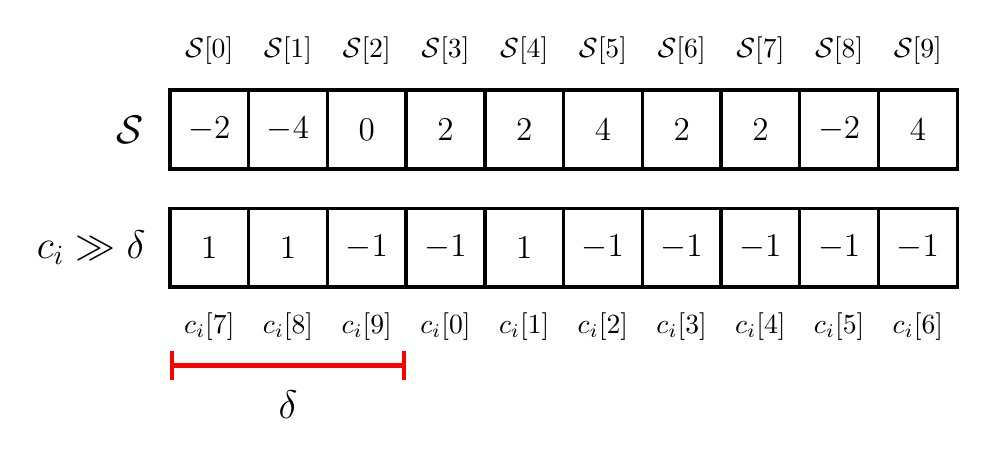
\begin{tikzpicture}
    % \draw[help lines] grid (20,7);

    % Sumsignal
    \begin{scope}[xshift=0cm,yshift=3cm]
        % Label
        \node[] (SS) at (-0.5,0.5) {\Large$\mathcal{S}$};

        % Cells and indices
        \foreach \x in {0,1,...,9} {
            \draw[black,very thick] (\x,0) rectangle (\x+1,1);
            \node[] at (\x+0.5,1.5) {$\mathcal{S}[\x]$};
        }

        % Values
        \foreach \x / \v in { 0/-2,1/-4,2/0,3/2,4/2,5/4,6/2,7/2,8/-2,9/4 } {
                
            \node[] at (\x+0.5,0.5) {\large$\v$};
            
        }
    \end{scope}

    % c_i
    \begin{scope}[xshift=0cm,yshift=1.5cm]
        % Label
        \node[] (ci) at (-1.0,0.5) {\Large$c_i \gg \delta$};

        % Cells
        \foreach \x in {0,1,...,9} {
            \draw[black,very thick] (\x,0) rectangle (\x+1,1);
        }

        % Indices
        \foreach \x in {0,1,...,6} {
            \node[] at (\x+3.5,-0.5) {$c_i[\x]$};
        }
        \foreach \x in {7,...,9} {
            \node[] at (\x-6.5,-0.5) {$c_i[\x]$};
        }

        % Values
        \foreach \x / \v in { 0/1,1/1,2/-1,3/-1,4/1,5/-1,6/-1,7/-1,8/-1,9/-1 } {
                
            \node[] at (\x+0.5,0.5) {\large$\v$};
            
        }

        % Delta vert line
        \draw[|-|,draw=red,ultra thick] (0,-1.0) -- (3,-1.0) 
            node[pos=0.5,below=5pt] {\Large$\delta$};
    \end{scope}

\end{tikzpicture}
\end{document}
